% !TeX root = ../thesis.tex

%%%%%%%%%%%%%%%%%%%%%%%%%%%%%%%%%%%%%%%%%%
\thesischapter[ch:feature]
  {``Why are there so many kinds of animals?''}
  {--- G. Evelyn Hutchinson, 1959}
  {Feature-level measures}
\nocite{hutchinson1959homage}
\chapterabstract{This chapter turns from aggregated community summaries to the analysis of individual microbial features. It distinguishes exploratory taxon-level analysis from comparative feature-level inference, where the aim is to identify taxa whose abundance or distribution differs between groups. Particular attention is given to the statistical complications caused by compositionality, sparsity, and heterogeneous library sizes. The chapter reviews common methodological approaches to differential abundance and differential distribution analysis and presents DACOMP and \texttt{waddR} as two permutation-based methods that are later combined with the \texttt{permApprox} framework to improve p-value resolution under limited permutation budgets.}
\chaptercontents

%%%%%%%%%%%%%%%%%%%%%%%%%%%%%%%%%%%%%%%%%%

%%%%%%%%%%%%%%%%%%%%%%%%%%%%%%%%%%%%%
\section{Introduction}
\label{sec:feature:intro}
%%%%%%%%%%%%%%%%%%%%%%%%%%%%%%%%%%%%%

Feature-level analysis investigates microbial taxa individually rather than through aggregated community summaries or network structures. Given a microbiome count matrix $X \in \mathbb{N}_0^{n \times p}$, the aim is to characterize or compare single features across samples, groups, or covariate patterns. This perspective provides a higher taxonomic resolution than community-level summaries because observed effects can be attributed to individual taxa. At the same time, it introduces additional statistical challenges, since feature-level analyses typically involve sparse, high-dimensional data and large numbers of simultaneous hypothesis tests.

Feature-related methods cover several related but distinct analysis tasks. In exploratory analyses, feature-level summaries are used to describe abundance, prevalence, and taxonomic patterns within a cohort. In comparative analyses, the objective is often to identify taxa whose abundance differs between groups, which is commonly referred to as differential abundance analysis. However, group differences may also involve changes in variability, zero structure, or distributional shape rather than shifts in abundance level alone. This motivates differential distribution analysis, where the full feature-specific distribution is compared across groups. A further class of feature-related methods uses microbial taxa as explanatory variables in regression or prediction models for sample-level outcomes. Such models also yield taxon-specific coefficients and therefore have a feature-level interpretation, but they address a different scientific question: whether the microbiome predicts or explains an external outcome.

In this thesis, we focus on differential abundance and differential distribution analysis. This choice reflects the aim of the application chapter, where early-life and birth-related variables are used to compare microbial profiles rather than to predict sample-specific outcomes from the microbiome. Regression models with microbial features as covariates would therefore reverse the direction of the main question. For example, they would ask whether the early microbiome predicts variables such as body mass index or other host characteristics, which is not the objective of the PASTURE analysis considered here. They are therefore acknowledged as part of the broader feature-level toolbox, but not developed further in this chapter.

The methodological focus on differential abundance and differential distribution analysis also serves a second purpose. Both approaches considered in detail in this chapter rely on permutation-based inference. DACOMP uses permutation testing for differential abundance analysis, while \texttt{waddR} uses permutation-based Wasserstein tests for differential distribution analysis. This makes both methods suitable for illustrating the finite-resolution problem of permutation p-values and for applying the \texttt{permApprox} framework developed in Chapter~\ref{ch:permapprox}. The emphasis is therefore not only on identifying taxon-specific group differences, but also on studying how permutation-based feature-level inference can be improved when only a limited number of permutations is computationally feasible.

The chapter first introduces exploratory taxon-level summaries and visualizations. It then discusses differential abundance analysis, gives an overview of common approaches, and presents DACOMP in more detail as the method used in the application chapter. Subsequently, differential distribution analysis is introduced, with a focus on the Wasserstein-based \texttt{waddR} framework and its adaptation to microbiome data. For both DACOMP and \texttt{waddR}, permutation-based inference is connected to the \texttt{permApprox} framework, which is used to refine small p-values under limited permutation budgets.

%%%%%%%%%%%%%%%%%%%%%%%%%%%%%%%%%%%%%
\section{Exploratory taxon-level analysis}
\label{sec:4feature:exploratory}
%%%%%%%%%%%%%%%%%%%%%%%%%%%%%%%%%%%%%

Exploratory feature-level analysis provides a first descriptive view of the individual microbial features observed in a microbiome study. While community-level summaries reduce each sample to diversity measures, dissimilarities, or multivariate model summaries, feature-level exploration keeps the taxonomic resolution explicit. The aim is not formal hypothesis testing, but rather to understand which features dominate the data set, how broadly they are observed across samples, and whether apparent patterns may depend on sparsity, taxonomic resolution, or a small number of highly abundant observations. Such analyses are therefore an important intermediate step between preprocessing and formal differential testing. They help to assess whether the chosen filtering, aggregation, and transformation steps are reasonable and provide context for interpreting later feature-wise results.

A basic summary at feature level is the abundance of each taxon. Depending on the analysis goal, abundance can be summarized by total read count, mean relative abundance, median relative abundance, or a transformed value such as a CLR coordinate. Total abundance highlights taxa that contribute strongly to the overall sequencing output, whereas mean or median relative abundance summarizes the relative contribution of a taxon across samples. However, these quantities can behave quite differently in sparse microbiome data. A taxon with high total abundance may occur in only a few samples, while a taxon with moderate abundance may be observed consistently across many samples. Abundance summaries should therefore usually be considered together with prevalence.

Prevalence describes the proportion of samples in which a taxon is observed, commonly defined as
\begin{equation}
\operatorname{prev}_i = \frac{1}{n}\sum_{k=1}^n I(x_{ki} > 0),
\end{equation}
where $I(\cdot)$ denotes the indicator function. Prevalence is particularly informative in sparse count matrices because it separates rare but occasionally abundant taxa from taxa that are consistently present. In practice, abundance and prevalence are often visualized jointly, for example in prevalence-abundance plots. Such plots can reveal whether the data contain a small number of highly prevalent dominant taxa, a long tail of rare taxa, or features that may be unstable targets for downstream inference. They also provide a transparent justification for prevalence- or abundance-based filtering rules.

Exploratory analyses may be performed at different taxonomic resolutions, such as ASV, genus, family, or phylum level. The choice of resolution depends on the aggregation strategy defined during preprocessing (Section~\ref{sec:2micro:aggregation}) and directly determines which features are summarized, visualized, and later tested. It is therefore important to interpret exploratory taxon-level patterns with respect to the chosen analysis unit. For example, a genus-level profile may be easier to interpret than an ASV-level profile, but it may also hide heterogeneous behavior among lower-level features that were aggregated into the same taxonomic group.

Visualization plays a central role in exploratory feature-level analysis. Stacked barplots of relative abundances provide a compact overview of dominant taxa and their variation across samples or groups. However, because only the most abundant taxa can usually be displayed, such plots should be interpreted as summaries of dominant composition rather than complete representations of the microbial community. Heatmaps of transformed abundances can reveal sample clusters, taxon-specific patterns, and outlying samples, especially when combined with taxonomic annotation or sample metadata. Boxplots or violin plots of selected taxa are useful for inspecting group-wise differences before formal testing, but their interpretation should account for the large number of zeros and the compositional nature of the data.

Importantly, exploratory taxon-level analysis should not be confused with statistical evidence for taxon-specific effects. Apparent differences in relative abundance may arise from compositional constraints, differences in library size, sparsity, or the behavior of other taxa. Similarly, visual patterns can be driven by a small number of samples or by the chosen transformation. The purpose of exploratory analysis is therefore to generate understanding and diagnostic insight, not to replace formal inference. In this thesis, exploratory feature-level analyses are used to characterize the taxonomic structure of the data, evaluate abundance and prevalence patterns, and guide the interpretation of subsequent differential abundance and differential distribution analyses.

%%%%%%%%%%%%%%%%%%%%%%%%%%%%%%%%%%%%%
\section{Differential abundance analysis}
\label{sec:4feature:diffabund}
%%%%%%%%%%%%%%%%%%%%%%%%%%%%%%%%%%%%%

Differential abundance analysis is one of the most widely used feature-level tasks in microbiome research. Its aim is to identify microbial features whose abundance differs between groups that are defined by sample variables such as clinical, environmental, or experimental characteristics. In the simplest two-group setting, each taxon $i = 1, \ldots, p$ is considered separately, and the question is whether its abundance pattern differs between the two groups. This feature-wise formulation makes differential abundance analysis attractive for biological interpretation because it can localize group differences to individual taxa. At the same time, it leads to a high-dimensional multiple testing problem and is strongly affected by the structural properties of microbiome data. As discussed in Chapter~2, microbiome sequencing data are sparse, overdispersed, and compositional. In particular, standard sequencing protocols provide relative rather than absolute abundance information, so that a change in the observed relative abundance of one taxon may reflect a change in that taxon itself, a change in other taxa, or a combination of both. Without additional information on absolute microbial load, differential abundance analysis must therefore be interpreted as inference on relative or compositional abundance patterns rather than direct inference on absolute microbial quantities.

Let $G_k \in \{0,1\}$ denote the group membership of sample $k$. For each taxon $i$, a differential abundance method defines a test statistic $T_i$ that compares the abundance pattern of taxon $i$ between the two groups, possibly after normalization, transformation, or reference-based adjustment. The corresponding feature-wise hypotheses can be written generically as
\begin{equation}
	H_{0i}: \text{taxon } i \text{ is not differentially abundant between the groups},
\end{equation}
against an alternative that taxon $i$ shows a group-associated abundance difference. The precise meaning of this null hypothesis depends on the chosen method. Some approaches formulate the null in terms of model parameters for observed counts, others in terms of transformed abundances, log-ratios, or contrasts relative to a reference set. This distinction is important because different methods may answer related but not identical statistical questions.

Figure~\ref{fig:4feature:overview_diff_abundance} illustrates this feature-wise workflow for DACOMP \citep{brill2022testing}: candidate taxa are compared separately between groups using DACOMP-rarefied counts, resulting in one permutation-based $p$-value per tested genus before multiple-testing correction.
The following subsection summarizes common classes of differential abundance methods before DACOMP is described in more detail as the method used in the application chapter.

\begin{figure}[H]
	\centering
	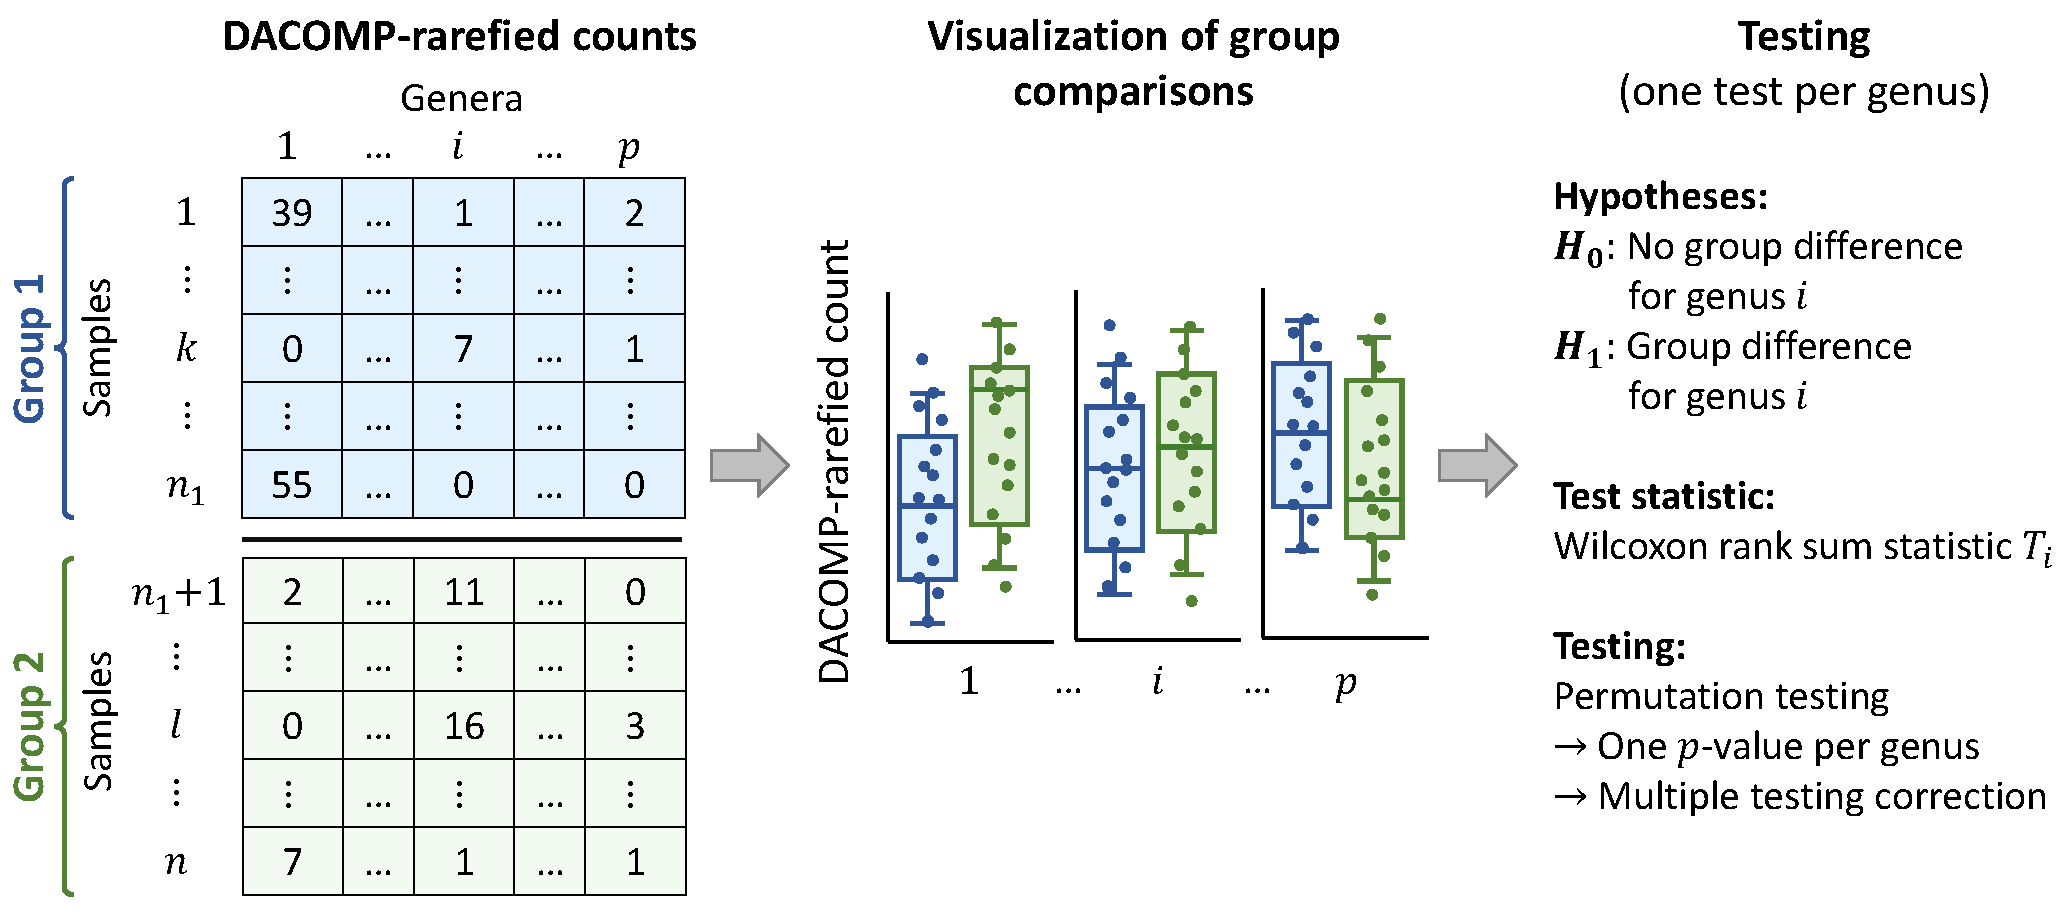
\includegraphics[width=\textwidth]{../ch04_feature_level/overview_figures/overview_diff_abundance.pdf}
	\caption{\textbf{Overview of differential abundance analysis with DACOMP.} DACOMP-rarefied counts are compared between groups separately for each tested genus. Group-wise distributions can be inspected descriptively, whereas formal inference is based on a taxon-specific Wilcoxon rank-sum statistic and a permutation test. This yields one $p$-value per genus, which is subsequently adjusted for multiple testing.}
	\label{fig:4feature:overview_diff_abundance}
\end{figure}

%====================================
\subsection{Overview of existing methods}
\label{sec:4feature:diffabund_overview}
%====================================

A large number of methods have been proposed for differential abundance analysis, reflecting the fact that no single modeling strategy resolves all statistical difficulties of microbiome data. A first group of methods adapts count-based models originally developed for RNA-seq data. Widely used examples include edgeR \citep{robinson2010edger}, DESeq2 \citep{love2014moderated}, and metagenomeSeq \citep{paulson2013differential}. These methods model taxon-specific counts and account for overdispersion, often through negative binomial or zero-inflated models combined with sample-specific normalization factors. Their main advantage is that they provide a well-established framework for high-dimensional count data, including variance estimation and multiple testing correction. However, their interpretation in microbiome applications depends strongly on the adequacy of the normalization strategy and on assumptions about the majority of features being unchanged across groups. Since microbiome data are compositional, such assumptions are not merely technical but affect the biological meaning of the resulting differential abundance calls.

A second group of methods is based more explicitly on compositional data analysis. These approaches start from the observation that only relative information is available and that taxon abundances should therefore be interpreted through ratios or log-ratios. ALDEx2 \citep{fernandes2014unifying}, for example, uses Monte Carlo instances drawn from a Dirichlet model and performs testing on centered log-ratio transformed values. ANCOM \citep{mandal2015analysis} evaluates log-ratios between taxa and identifies features whose ratios to many other features differ between groups. These methods reduce the risk of detecting spurious effects caused by the constant-sum constraint, but they also make explicit that differential abundance in relative data is inherently comparative: a taxon is not assessed in isolation, but relative to other taxa or to a chosen reference structure.

More recent methods further refine this idea by estimating bias terms, selecting reference features, or formulating differential abundance in terms of compositional contrasts. ANCOM-BC \citep{lin2020analysis} introduces a bias-correction framework to account for sampling fractions, while LinDA \citep{zhou2022linda} uses linear models on centered log-ratio transformed data and aims to correct the compositional bias under sparsity. DACOMP \citep{brill2022testing} follows a reference-based strategy and performs differential abundance testing after selecting a set of taxa assumed to be non-differential. These methods differ in how they define the target of inference, how they handle the compositional constraint, and whether inference is based on asymptotic approximations, model-based assumptions, or resampling procedures.

Comparative studies have shown that differential abundance methods can yield substantially different results on the same data set, and that their performance depends on characteristics such as sparsity, sample size, effect size distribution, library size variability, and the proportion of truly differential taxa \citep{weiss2017normalization,nearing2022microbiome}. This variability is not surprising because different methods encode different assumptions about the data-generating process and about what it means for a taxon to be differentially abundant. Consequently, the choice of method should be guided by the scientific question, the data structure, and the intended interpretation of the results rather than by software availability alone.

In this thesis, the focus is on differential abundance analysis as a feature-wise comparative task under compositional constraints. For the application in Chapter~7, DACOMP is used because it explicitly addresses compositionality through a reference-based construction and relies on permutation-based inference. This makes it particularly suitable for connecting feature-level microbiome testing with the \texttt{permApprox} framework developed in Chapter~6. After introducing DACOMP in the next subsection, we describe how small DACOMP p-values can be refined using \texttt{permApprox} to reduce the finite-resolution limitations of empirical permutation testing.

%====================================
\subsection{DACOMP}
\label{sec:4feature:dacomp}
%====================================

DACOMP is a differential abundance method designed for compositional count data with potentially many zero counts \citep{brill2022testing}. In contrast to log-ratio based approaches such as the CLR transformation, DACOMP does not first transform the full composition into log-ratio coordinates. Instead, it accounts for compositionality through a reference-based testing strategy. The method is implemented in the \texttt{dacomp} R package and is based on the idea that differential abundance of an individual taxon cannot be inferred from its raw counts alone. As discussed in Chapter~\ref{ch:microbiome}, the total sequencing depth in microbiome data is arbitrary and the observed counts of all taxa are constrained to sum to this depth. Thus, an apparent change in the count or relative abundance of one taxon may be caused by a change in that taxon, by changes in other taxa, or by the compositional constraint itself. DACOMP addresses this problem by testing each candidate taxon relative to a set of reference taxa that are assumed to be non-differential with respect to the phenotype or group variable. These reference taxa serve as an internal comparison background, so that the candidate taxon is evaluated relative to taxa that are assumed to be stable rather than relative to the full sample total.

The reference set $\mathcal{B}$ is constructed from the data by identifying taxa whose log-ratios relative to all other taxa vary only weakly across samples. Let $X = (X_{ki}) \in \mathbb{N}_0^{n \times p}$ denote the count matrix, where $X_{ki}$ is the count of taxon $i$ in sample $k$. For each taxon~$i$, DACOMP considers pairwise log-ratios of the form
\begin{equation}
	\log_{10}\!\left(\frac{X_{ki}+1}{X_{k\ell}+1}\right), \qquad \ell \neq i,
	\label{eq:4feature:dacomp_log_ratios}
\end{equation}
where the pseudo-count avoids undefined ratios in the presence of zeros. The variability of these log-ratios across samples is summarized by a score $S_i$. Taxa with $S_i \leq S_{\mathrm{crit}}$ are selected as reference taxa, where $S_{\mathrm{crit}}$ is chosen such that the total number of reference reads per sample remains in a practical range. In this way, DACOMP aims to construct a reference set that is sufficiently stable across samples while still large enough to support the subsequent rarefaction-based testing procedure.

\newpage
For a candidate taxon $i \notin \mathcal{B}$, DACOMP compares the abundance of taxon $i$ with the total abundance of the reference taxa. Let
\begin{equation}
	R_k = \sum_{\ell \in \mathcal{B}} X_{k\ell}
	\label{eq:4feature:dacomp_reference_abundance}
\end{equation}
denote the total reference abundance in sample $k$. DACOMP then defines the common rarefaction depth
\begin{equation}
	\lambda = \min_{1 \leq k \leq n} R_k.
	\label{eq:4feature:dacomp_rarefaction_depth}
\end{equation}
For each sample $k$, a rarefied count $Z_{ki}$ is generated by sampling $\lambda$ reads without replacement from the pool consisting of taxon $i$ and the reference taxa. Equivalently, writing the hypergeometric distribution in terms of population size, number of candidate-taxon reads, and number of draws,
\begin{equation}
	Z_{ki} \sim \operatorname{Hypergeometric}\!\left(X_{ki}+R_k, X_{ki}, \lambda\right).
	\label{eq:4feature:dacomp_rarefied_counts}
\end{equation}
The rarefaction step places samples on a comparable scale with respect to the reference taxa and avoids relying on a parametric model for the original count distribution.

The feature-wise test statistic is then computed from the rarefied counts. In the two-group setting, let $Y_k \in \{0,1\}$ denote the group label of sample $k$. DACOMP uses the Wilcoxon rank-sum statistic
\begin{equation}
	T_i = \sum_{k:Y_k = 1} \operatorname{rank}(Z_{ki})
	\label{eq:4feature:dacomp_test_statistic}
\end{equation}
to compare the rarefied counts between groups. The corresponding null hypothesis can be formulated as
\begin{equation}
	H_{0i}: \text{taxon } i \text{ is not differentially abundant relative to the reference set } \mathcal{B}.
	\label{eq:4feature:dacomp_null}
\end{equation}
Because the test is based on ranks of rarefied counts, DACOMP avoids specifying a full parametric model for the taxon counts. This is advantageous in microbiome data, where sparsity, overdispersion, and excess zeros make simple distributional assumptions difficult to justify.

Inference is performed by permutation of the group labels. For each taxon $i$, the observed statistic $T_i$ is compared with a permutation distribution $\{T_i^{*(b)}\}_{b=1}^B$ obtained by repeatedly shuffling the labels $Y_k$ and recalculating the statistic. This yields empirical permutation p-values for all candidate taxa. The use of permutation testing makes DACOMP flexible and well suited to the feature-wise comparative setting considered in this thesis. At the same time, the resulting p-values are limited by the finite number of permutations: with $B$ permutations, empirical p-values lie on a discrete grid, which can be restrictive after multiple testing correction. This limitation is addressed in Chapter~\ref{ch:permapprox}, where the \texttt{permApprox} framework is introduced for refining small permutation p-values. Since \texttt{dacomp} exports both the observed statistic $T_i$ and the permuted statistics $\{T_i^{*(b)}\}_{b=1}^B$, its output can be used directly as input for \texttt{permApprox}. In the application chapter, DACOMP is therefore used for differential abundance testing, and small permutation p-values are refined with \texttt{permApprox} as a post-processing step.

%%%%%%%%%%%%%%%%%%%%%%%%%%%%%%%%%%%%%
\section{Differential distribution analysis}
\label{sec:4feature:diffdist}
%%%%%%%%%%%%%%%%%%%%%%%%%%%%%%%%%%%%%

\begin{figure}[H]
	\centering
	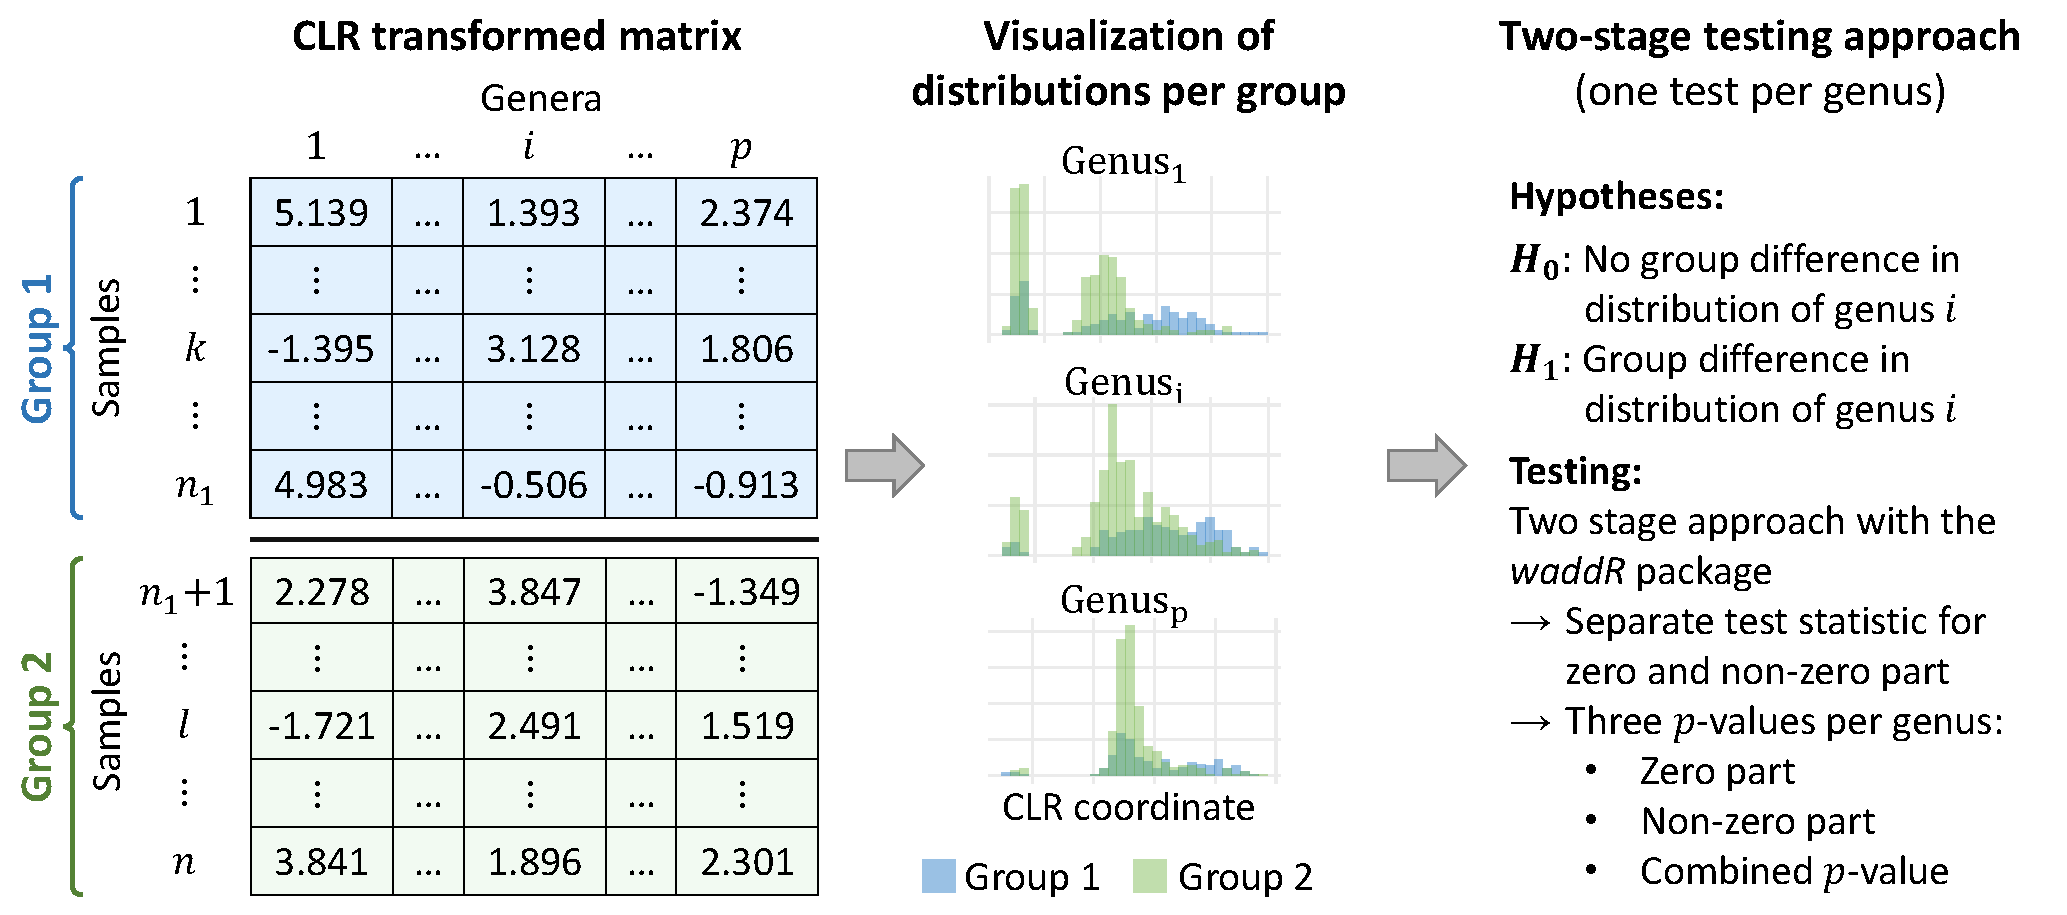
\includegraphics[width=\textwidth]{../ch04_feature_level/overview_figures/overview_diff_distribution.pdf}
	\caption{\textbf{Overview of differential distribution analysis with \texttt{waddR}.} For each genus, the group-specific distributions of CLR-transformed values are compared. The \texttt{waddR} framework separates differences in the frequency of observed zeros from differences in the distribution of CLR values among samples with positive original counts. The resulting zero-part and non-zero-part $p$-values can be combined into an overall $p$-value for each tested genus.}
	\label{fig:4feature:overview_diff_distribution}
\end{figure}

Differential abundance analysis aims to identify taxa whose abundance levels differ between groups. In many applications, however, group differences may go beyond a shift in mean or median abundance. A taxon may have similar average abundance in two groups but differ in variability, zero frequency, skewness, multimodality, or other aspects of distributional shape. Such differences can be biologically relevant, for example when a taxon is consistently present in one group but occurs only in a subset of individuals in another group. Differential distribution analysis therefore asks the more general question of whether the full feature-specific distribution differs between groups.
Figure~\ref{fig:4feature:overview_diff_distribution} illustrates this feature-wise perspective for the two-stage \texttt{waddR} framework, which separately considers differences in zero frequencies and in the distributions of non-zero CLR values.

For taxon $i$, let $F_i^{(1)}$ and $F_i^{(2)}$ denote the distributions of the preprocessed abundance values in the two groups with sample sizes $n_1$ and $n_2$. Differential distribution analysis considers the null hypothesis
\begin{equation}
\label{eq:4feature:diffdist_null}
H_{0i}: F_i^{(1)} = F_i^{(2)}.
\end{equation}
This null hypothesis is broader than a null hypothesis on a single location parameter. It is violated not only by differences in mean abundance, but also by differences in variance, zero structure, tail behavior, or modality. The price of this broader alternative is that distributional tests may be less specific: a significant result indicates that the distributions differ, but does not automatically identify which aspect of the distribution is responsible.

Compared with differential abundance analysis, differential distribution analysis is less standardized in microbiome research. The following subsection therefore briefly reviews classical distributional two-sample tests and more recent approaches developed for high-throughput single-cell data. The subsequent subsection then focuses on \texttt{waddR}, which is used in the application chapter and is particularly relevant for this thesis because of its connection to permutation testing and GPD-based p-value approximation.

%====================================
\subsection{Overview of existing methods}
\label{sec:4feature:diffdist_overview}
%====================================

Classical nonparametric two-sample tests already provide tools for testing equality of one-dimensional distributions. A prominent example is the two-sample Kolmogorov--Smirnov test \citep{kolmogorov1933sulla,smirnov1948table}. Let $\hat F_i^{(1)}$ and $\hat F_i^{(2)}$ denote the empirical distribution functions of taxon $i$ in the two groups. The Kolmogorov--Smirnov statistic is defined as
\begin{equation}
\label{eq:ks_statistic}
D_i = \sup_x \left| \hat F_i^{(1)}(x) - \hat F_i^{(2)}(x) \right|.
\end{equation}
It measures the largest vertical distance between the two empirical cumulative distribution functions. The test is sensitive to localized discrepancies between distributions and is distribution-free under continuity assumptions. However, microbiome data often contain many ties and zeros, so the usual continuous-distribution theory is not directly applicable. In such settings, permutation-based p-values are more appropriate, but they again inherit the finite-resolution problem discussed in Chapter~\ref{ch:permapprox}.

Other classical tests compare empirical distribution functions through integrated rather than supremum-type distances. Cramér--von Mises-type statistics integrate squared differences between distribution functions \citep{cramer1928composition,vonmises1928wahrscheinlichkeit}, while Anderson--Darling-type tests use a weighting that gives more emphasis to tail differences \citep{anderson1952asymptotic}. These tests are also designed to detect general distributional differences, but their interpretation remains global: they test whether the distributions differ without directly separating location, scale, and shape effects.

More recent differential distribution methods have been developed mainly in the context of single-cell data analysis, where full expression distributions across cells are of scientific interest. The method \texttt{scDD}, for example, uses a Bayesian mixture modeling framework to classify genes according to different types of distributional changes, including changes in modality and in the proportions of cells assigned to expression components \citep{korthauer2016statistical}. The method \texttt{distinct} provides a general framework for differential distribution analysis that is particularly suited to single-cell and cytometry data, where differences may occur in complex distributional features rather than only in mean expression \citep{tiberi2023distinct}. These methods illustrate that distributional testing is useful when heterogeneity itself is part of the biological signal.

Among the more specialized approaches, \texttt{waddR} provides a Wasserstein-based framework for testing differential distributions \citep{schefzik2021fast}. In contrast to the Kolmogorov--Smirnov statistic, which is based on the maximum distance between empirical distribution functions, the 2-Wasserstein distance compares distributions through their quantile functions. For two one-dimensional distributions $F_i^{(1)}$ and $F_i^{(2)}$, the squared 2-Wasserstein distance can be written as
\begin{equation}
\label{eq:wasserstein_distance}
W_2^2\left(F_i^{(1)},F_i^{(2)}\right) = \int_0^1 \left( \left(F_i^{(1)}\right)^{-1}(u) - \left(F_i^{(2)}\right)^{-1}(u) \right)^2 \, \mathrm{d}u.
\end{equation}
This distance has an intuitive interpretation as the amount of transport required to transform one distribution into the other. Moreover, in one dimension, the squared 2-Wasserstein distance admits a decomposition into location, size, and shape components. The decomposition separates contributions related to location, variability, and residual shape differences after centering and scaling. This decomposition is useful because it provides more insight into the nature of a detected distributional difference than a single global p-value alone.

Although methods such as \texttt{scDD}, \texttt{distinct}, and \texttt{waddR} were primarily motivated by single-cell applications, the statistical question they address is not restricted to single-cell data. They can also be considered for microbiome feature-level analysis when the aim is to test whether the distribution of a taxon differs between groups beyond a simple abundance shift. In this thesis, we focus on \texttt{waddR} for two reasons. First, it provides a direct feature-wise test for equality of one-dimensional distributions and decomposes the squared 2-Wasserstein distance into interpretable components. Second, the workflow already includes a generalized Pareto distribution (GPD) approximation for small permutation p-values. This makes \texttt{waddR} particularly suitable for comparison with the constrained GPD-based p-value refinement developed in Chapter~\ref{ch:permapprox}.

%====================================
\subsection{Two-stage differential distribution testing with \texttt{waddR}}
\label{sec:4feature:diffdist_waddr}
%====================================

The \texttt{waddR} approach provides a Wasserstein-based framework for testing differential distributions in high-throughput data \citep{schefzik2021fast}. For each feature, the method compares the distributions observed in two groups using the squared 2-Wasserstein distance. As introduced above, this distance compares one-dimensional distributions through their quantile functions and therefore captures differences in the full distribution rather than only differences in a location parameter. This makes \texttt{waddR} particularly suitable for settings in which group differences may involve changes in variability, zero frequency, or distributional shape.

A specific feature of \texttt{waddR} is its two-stage testing strategy for data with excess zeros. In the original single-cell setting, the first stage tests for differential proportions of zero observations between the two groups. This idea follows \texttt{scDD}: for each gene, a logistic regression model\footnote{The \texttt{waddR} paper refers to this step as Bayesian logistic regression. Since the cited \texttt{scDD} description formulates the zero test as logistic regression adjusted for cellular detection rate, we describe the step here in terms of the underlying regression model.} is fitted to the binary zero indicator and adjusted for the cellular detection rate, which accounts for differences in the number of detected genes per cell \citep{finak2015mast,korthauer2016statistical}. 

Let
\begin{equation}
\label{eq:waddr_zero_prob}
\pi_i^{(g)} = \Pr\left(X_i^{(g)} = 0\right), \qquad g \in \{1,2\},
\end{equation}
denote the group-specific zero probabilities for feature $i$. The corresponding null hypothesis is
\begin{equation}
\label{eq:waddr_zero_null}
H_{0i,0}: \pi_i^{(1)} = \pi_i^{(2)}.
\end{equation}
The zero stage yields a p-value $p_{i,0}$. We denote the corresponding Wald statistic for the group effect in the logistic regression model by $Z_{i,0}$.

The second stage restricts the analysis to the non-zero observations and tests whether their distributions differ between groups. Let $F_{i,+}^{(1)}$ and $F_{i,+}^{(2)}$ denote the group-specific distributions of the positive values of feature $i$. The corresponding null hypothesis is
\begin{equation}
\label{eq:waddr_nonzero_null}
H_{0i,+}: F_{i,+}^{(1)} = F_{i,+}^{(2)}.
\end{equation}
The test statistic for the non-zero stage is the squared 2-Wasserstein distance
\begin{equation}
\label{eq:4feature:waddr_nonzero_statistic}
T_{i,+} = W_2^2\left(F_{i,+}^{(1)},F_{i,+}^{(2)}\right).
\end{equation}
Large values of $T_{i,+}$ indicate stronger evidence against equality of the non-zero distributions. This stage yields a p-value $p_{i,+}$ for differential distributions among the non-zero observations.

The two p-values from the zero and non-zero parts can be combined into an overall p-value using Fisher's method \citep{fisher1925statistical}. For feature $i$, the Fisher statistic is
\begin{equation}
\label{eq:waddr_fisher}
C_i = -2\left(\log p_{i,0} + \log p_{i,+}\right).
\end{equation}
Under the classical Fisher combination framework, and assuming independence of the two component p-values under the joint null hypothesis, $C_i$ is compared with a chi-squared distribution with four degrees of freedom, leading to a combined p-value
\begin{equation}
\label{eq:4feature:waddr_combined_pvalue}
p_{i,\mathrm{comb}} = \Pr\left(\chi^2_4 \geq C_i\right).
\end{equation}
The resulting p-value summarizes evidence from both components, while the separate p-values retain information about whether the signal is driven by zero frequency, non-zero distributional differences, or both.

%====================================
\subsection{Adaptation of \texttt{waddR} to microbiome data}
\label{sec:4feature:diffdist_waddr_microbiome}
%====================================

In principle, \texttt{waddR}'s two-stage idea is also relevant for microbiome data, where zeros are frequent and may carry biological or technical information. However, the original \texttt{waddR} implementation assumes non-negative expression values. In its two-stage wrapper, non-zero observations are identified by retaining values larger than zero. This is appropriate for count-like single-cell expression data, but it is not appropriate after CLR transformation, where negative values simply indicate below-geometric-mean relative abundance rather than absence.

For microbiome data, we therefore use an adapted two-stage strategy. The count matrix is first transformed to relative abundances, zeros are handled by multiplicative replacement, and the resulting strictly positive compositions are transformed using the CLR transformation, following the preprocessing choices in Section~\ref{sec:2micro:preprocessing_choices_thesis}. The zero stage is nevertheless defined on the original count scale: a sample is treated as zero for taxon $i$ if the original count of that taxon is zero. The zero-stage p-value $p_{i,0}$ therefore tests for differences in original zero frequencies between groups.

For the non-zero Wasserstein stage, zeros are again defined on the original count scale, but the tested values are taken from the CLR-transformed matrix. Thus, for each taxon, we retain samples with positive original counts and compare the corresponding CLR values between groups. Let $Z_i$ denote the CLR-transformed coordinate of taxon $i$, and let $F_{i,+}^{(g)}$ denote the distribution of $Z_i^{(g)}$ among samples with $X_i^{(g)} > 0$. The non-zero null hypothesis remains
\begin{equation}
H_{0i,+}: F_{i,+}^{(1)} = F_{i,+}^{(2)},
\end{equation}
but it is now interpreted as equality of the CLR-transformed distributions among originally observed values. Negative CLR values are retained whenever the original count is non-zero. This preserves the two-stage interpretation while avoiding the erroneous removal of negative CLR coordinates.

For the non-zero part, we use the semi-parametric Wasserstein permutation test implemented in \texttt{waddR}. For each feature $i$, the observed statistic $T_i$ is compared with a permutation distribution $\{T_i^{*(b)}\}_{b=1}^B$ obtained by shuffling the group labels and recalculating the Wasserstein statistic in \eqref{eq:4feature:waddr_nonzero_statistic}. Since permutation testing can become computationally demanding when many features are tested, \texttt{waddR} provides a semi-parametric p-value approximation based on the generalized Pareto distribution for small permutation p-values. This is directly connected to the finite-resolution problem discussed in Chapter~\ref{ch:permapprox}: with a limited number of permutations, empirical p-values are restricted to a coarse grid and may be insufficiently resolved in the tail.

In the application in Chapter~\ref{ch:application}, the GPD approximation used by \texttt{waddR} produced many zero p-values for the non-zero distributional test. Such zero p-values are problematic for the reasons discussed in Chapter~\ref{ch:permapprox}: they are not valid permutation p-values, remain zero after multiple testing correction, and prevent a meaningful ranking of very strong signals. The aim of the \texttt{permApprox} refinement in this setting is therefore not primarily to compare GPD-based p-values with empirical permutation p-values. Rather, the central question is whether the constrained GPD approach implemented in \texttt{permApprox} can eliminate zero p-values while preserving the Wasserstein-based test statistic used by \texttt{waddR}.

A practical complication is that the original \texttt{waddR} output does not provide the complete matrix of permuted test statistics required by \texttt{permApprox}. The \texttt{permApprox} workflow requires, for each tested feature, the observed statistic $T_i$ together with the permutation statistics $\{T_i^{*(b)}\}_{b=1}^B$. We therefore use a modified R implementation of the \texttt{waddR} approach that exports these quantities for the non-zero distributional test. The exported observed and permuted Wasserstein statistics are then passed to \texttt{permApprox}, where p-values are recomputed using the constrained GPD-based refinement described in Chapter~\ref{ch:permapprox}.

Only the non-zero Wasserstein part is refined with \texttt{permApprox}. The zero-proportion p-value is kept separate and can be combined with the refined non-zero p-value using Fisher's method. This preserves the interpretability of the two-stage procedure while adapting it to compositional microbiome data: original counts determine zero status, CLR-transformed values define the non-zero distributions, and \texttt{permApprox} refines the permutation-based tail inference for the Wasserstein statistic.
